\documentclass{article}

%............Inicia Preambulo.......................
\usepackage{graphicx}
\usepackage{float}
\usepackage[utf8]{inputenc}
\usepackage[shortlabels]{enumitem}
\usepackage{textcomp}
\usepackage{multicol}
\usepackage{caption}
\usepackage[spanish]{babel}
\usepackage[total={17.5cm, 23cm}, top=2cm, left=2cm]{geometry}
\usepackage{esvect}
\usepackage[font=footnotesize]{caption}

\spanishdecimal{.}
\parindent 0cm

%.............Fin de Preambulo........................

\begin{document}

\begin{center}
{\Large \textbf{Universidad Autónoma de Coahuila}}
\end{center}

\begin{center}
{\large Facultad de Ciencias Físico-Matemáticas}
\end{center}

%Materia
\begin{center}
{\large Metodos Numericos}
\end{center}

%Título
\begin{center}
{\large Metodo de Horner}
\end{center}

%Fecha
\begin{center}
{\large 29 de Noviembre del 2019}
\end{center}

%Autor
\begin{center}
{\large José Antonio Olveda García}
\end{center}

\vspace{5mm}

\begin{multicols}{2}

\section{Objetivo}
\label{sec:obj}
  El objetivo de este programa es resolver los polinomios por medio del metodo de Horner o del metodo de la division sintetica.

\section{Introduccion}
\label{sec:Intro}
Consiste en calcular el cociente y el resto de la division de polinomios, operando unicamente con coeficientes.
\\
\\
\textbf{¿En que caso se aplica?}
\\
Es un metodo general, se aplica para dividir polinomios de cualquier grado, pero se aconseja su uso cuando el divisor es mayor o igual que 2.
\\
\\
La evaluacion usando la forma monomial del polinomio de grado n requiere al menos n sumas y $\frac{n_{2}+n}{2}$ multiplicaciones, si las potencias se calculan mediante la repeticion de multiplicaciones.
\section{Metodologia}
\label{sec:Met}
Sea un polinomio de grado n
\begin{equation}
P_{n}(x)=a_{0}x^{n}+a_{1}x^{n-1}+...+a_{n-1}x+a_{n}
\end{equation}
Un polinomio $P_{n}(x)$ de grado n \textbf{tiene n ceros} (algunos o todos pueden ser complejos)

\begin{equation}
P(x)=a_{0}(x-x_{0})^{m_{1}}x-x_{2})^{m_{2}}...x-x)^{m_{k}}
\end{equation}

\begin{equation}
\sum_{i=1}^{k}=m_{k}=n
\end{equation}

Ejemplo
\\
\begin{center}
$2x^{2}+6x+4=2(x+1)(x+2)$
\end{center}
Ejemplo de aplicacion del metodo de Horner
\\
\\
Sea el polinomio $P(x)=2x^{4}-3x^{2}+3x-4$
\begin{figure}[H]
\centering
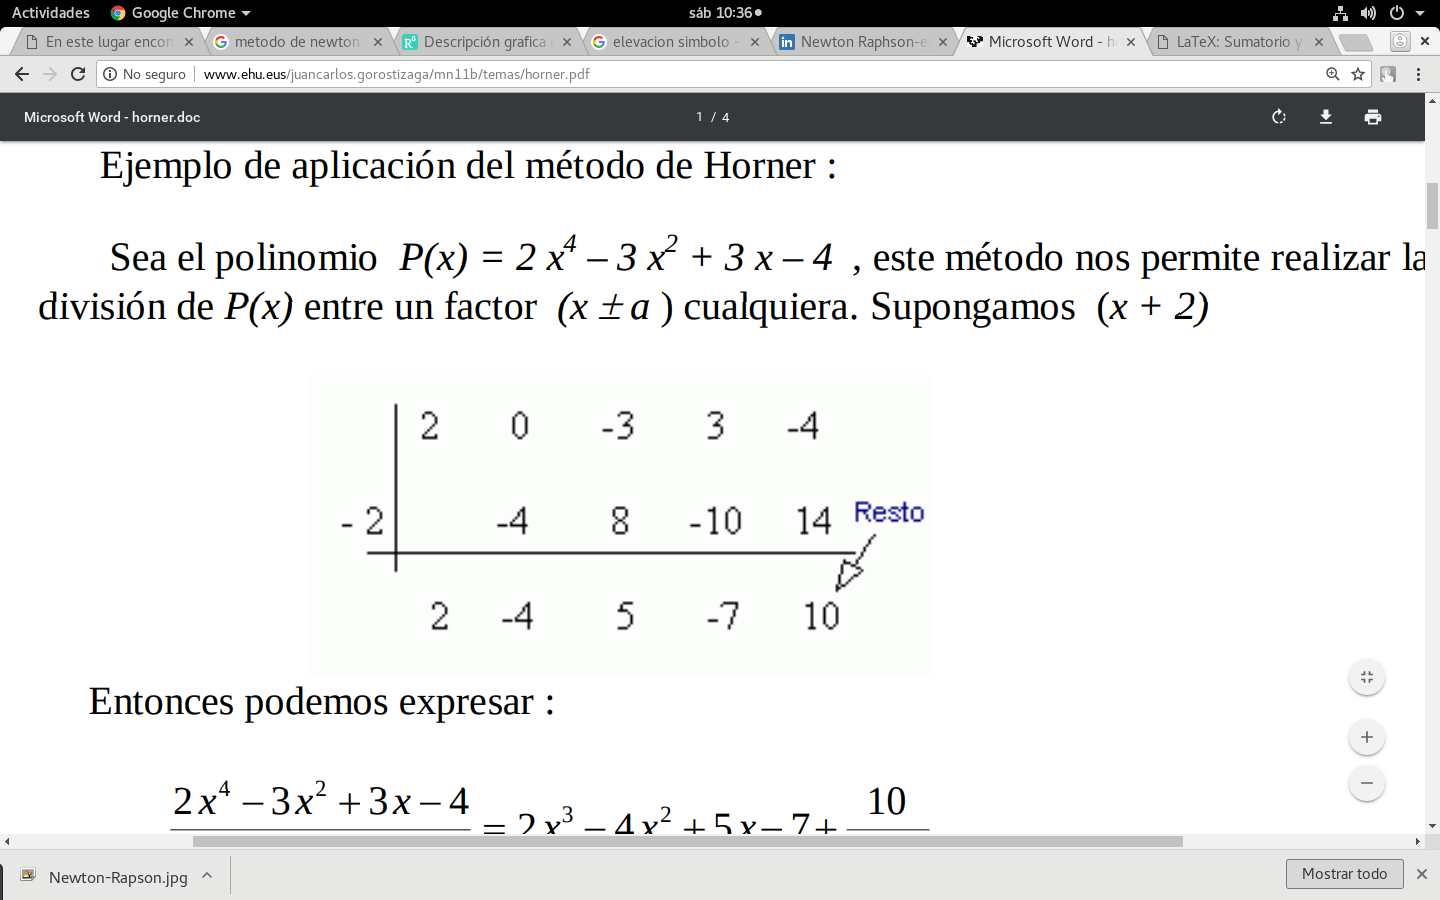
\includegraphics[scale=.25, %
trim=250 250 500 350,clip]{DivisionSintetica.png}
\caption{Division Sintetica 1}
\end{figure}

Entonces podemos expresar:
\begin{equation}
\frac{2x^{4}-3x^{2}+3x-4}{x+2} = 2x^{3}-4x^{2}+5x-7+\frac{10}{x+2}
\end{equation}
O bien
\begin{center}
$(x+2)(2x^{3}-4x^{2}+5x-7)+10$
\\
$P(-2)=10$
\end{center}




\section{Descripcion del metodo de Horner}
\label{sec:Des}
Sea un polinomio 
\begin{equation}
P(x)=a_{0}x^{n}+a_{1}x^{n-1}+...+a_{n-1}x+a_{n}
\end{equation}

Se toman 
\\
$d_{0}=a_{0}$
\\
$d_{k}=a_{k}+a_{k-1}x_{0}(k=1,...,n-1)$
\\
$d_{n}=P(x_{0})$
\\
Asi el cociente de hacer  $\frac{P(x)}{x-x_{0}}$ es:
\\
\begin{center}
$Q(x)=d_{0}x^{n-1}+d_{1}x^{n-1}+...+d_{n-1}$
\end{center}
Las ventajas del metodo de Horner son:

Podemos expresar un polinomio en forma
\begin{center}
P(x)=(x-$x_{0}$)Q(x)+$d_{n}$
\end{center}

Al derivar la anterior expresion, tenemos 
\begin{center}
P'(x)=Q(x)+($x-x_{0}$)Q'(x)
\end{center}
Es decir. P'($x_{0}$)=Q($x_{0}$)

\section{Ventajas y Desventajas}
\label{sec:Ven}
\textbf{Ventajas}
\\
1. Es optimo para programar debido a que solo maneja puros coeficientes.
\\
2. Es facil y rapido
\\
\\
\textbf{Desventajas}
\\
1. Una vez teniendo un grado bastante elevado torna a hacerse bastante complicado y  puede obtenerse un error.
\section{Implementacion del programa}
\label{sec:Imp}
En este caso se realizo una funcion del metodo de horner para asi simular el efecto de la division sintetica, donde comprobaremos si el resultado es correcto a partir del siguiente ejemplo
\begin{equation}
P(x)=2x^{4}-3x^{2}+3x-4
\end{equation}
con $x_{0}=-2$
Aplicando el programa, veremos si la aproximacion cumple
\begin{figure}[H]
\centering
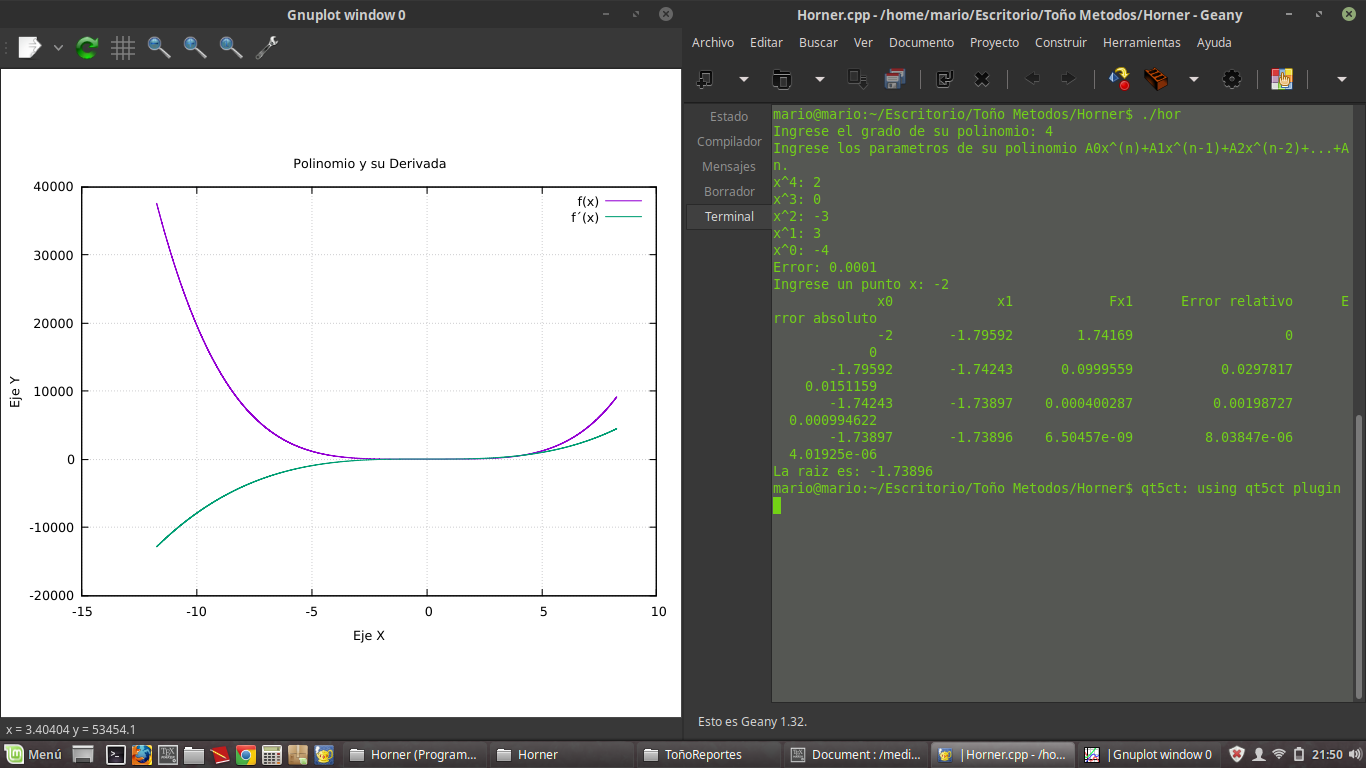
\includegraphics[scale=.125]{Horner.png}
\caption{Metodo de Horner implementado como programa}
\end{figure}
Mostrando asi que mi nueva aproximacion es de 1.796, la cual es correcta, dicha aproximacion presentada, ademas de añadir una grafica donde muestra la funcion presentada, y que es lo que hace

\section{Conclusiones}
\label{sec:Conclu}
Este metodo que acabamos de mencionar es importante porque nos permite dividir dos polinomios de cualquier grado para obtener especialmente el cociente y el residuo de la division.
\end{multicols}

\end{document}